\documentclass{article}
\usepackage[fleqn]{amsmath}
\usepackage{amssymb,graphicx,color,graphicx,slashed, microtype, parskip, enumitem, extarrows, needspace}
%\usepackage[utf8x]{inputenc}
\usepackage[top=1.5cm, bottom=1.5cm, right=6cm, left=1.5cm, heightrounded, marginparwidth=5cm, marginparsep=0.5cm]{geometry}

\hbadness = 10000
\hfuzz=100pt 
    
\usepackage{marginnote}
\renewcommand*{\marginfont}{\footnotesize}

\usepackage{hyperref}
\hypersetup{colorlinks=true, urlcolor=NavyBlue, bookmarksdepth=3}

\makeatletter\newcommand{\@minipagerestore}{\setlength{\parskip}{\medskipamount}}\makeatother

% =============== Index ===========================

\usepackage[nonewpage]{imakeidx}
\makeindex

% =============== Color Definitions ===============
    
\usepackage[svgnames]{xcolor}
\colorlet{ColorTitle}{Black}
\colorlet{ColorSectionName}{Black}
\colorlet{ColorBoxFG}{Gray}
\colorlet{ColorBoxText}{Black}
\colorlet{ColorBoxBG}{White}


% =============== Title Style ===============
    
\usepackage{titling} % Allows custom title configuration
    
\newcommand{\HorRule}{\color{ColorTitle}\rule{\linewidth}{1pt}} % Defines the gold horizontal rule around the title
    
\pretitle{
    \vspace{-50pt} % Move the entire title section up
    \HorRule\vspace{9pt} % Horizontal rule before the title
    \fontsize{27}{36}\usefont{OT1}{phv}{b}{n}\selectfont
    \color{ColorTitle} % Text colour for the title and author(s)
}
    
\posttitle{\par\vskip 15pt} % Whitespace under the title
    
\preauthor{\fontsize{17}{0}\usefont{OT1}{phv}{m}{n}\selectfont\color{ColorTitle}} % Anything that will appear before \author is printed
    
\postauthor{\par\HorRule}

\newcommand{\COURSENAME}{\href{http://phyw.people.ust.hk/teaching/PHYS2022-2015/}{\textcolor{black}{PHYS 2022}}}
\newcommand{\YW}{\href{http://phyw.people.ust.hk/}{\textcolor{black}{Yi Wang}}}
\newcommand{\PHYS}{\href{http://physics.ust.hk}{\textcolor{black}{Department of Physics}}}
\newcommand{\HKUST}{\href{http://www.ust.hk/}{\textcolor{black}{HKUST}}}
\author{\COURSENAME, \YW, \PHYS, \HKUST}

\date{}

% =============== Section Name Style ===============
    
\usepackage{titlesec}
    
\titleformat{\section}
    {\fontsize{15}{20}\usefont{OT1}{phv}{b}{n}\color{ColorSectionName}}
    {\thesection}{1em}{}
    %[{\vspace{0.2cm}\titlerule[0.8pt]}]
    
\titleformat{\subsection}
    {\fontsize{14}{20}\usefont{OT1}{phv}{m}{n}\color{ColorSectionName}}
    {\thesubsection}{1em}{}
    
\titleformat{\subsubsection}
    {\fontsize{12}{20}\usefont{OT1}{phv}{m}{n}\color{ColorSectionName}}
    {}{0em}{}
      
\setcounter{secnumdepth}{4}
        
% =============== Box Style ===============
    
\usepackage[most]{tcolorbox}
    
\newtcolorbox{tbox}[1]{
    colback=ColorBoxBG, colframe=ColorBoxFG, coltext=ColorBoxText,
    sharp corners, enhanced, breakable, parbox=false,
    before skip=1em, after skip=1em,
    title={#1}, fonttitle=\usefont{OT1}{phv}{b}{n}, 
    attach boxed title to top left={yshift=-0.1mm}, boxed title style={sharp corners, colback=ColorBoxFG, left=0.405cm},
    rightrule=-1pt,toprule=-1pt, bottomrule=-1pt
}

\newtcolorbox{mtbox}[1]{
    colback=ColorBoxBG, colframe=ColorBoxFG, coltext=ColorBoxText,
    sharp corners, enhanced, breakable, parbox=false,
    before skip=1em, after skip=1em,
    title={#1}, fonttitle=\usefont{OT1}{phv}{b}{n},
    attach boxed title to top left={yshift=-0.1mm}, boxed title style={sharp corners, colback=ColorBoxFG, left=0.15cm},
    rightrule=-1pt,toprule=-1pt, bottomrule=-1pt, 
    left=0.5em
}

% =============== tikz has to be loaded after xcolor
\usepackage{tikz}

\newcommand*\enumlabel[1]{\tikz[baseline=(char.base)]{
			\node[shape=rectangle,inner sep=2pt,fill=ColorBoxFG] (char) 
			{\fontsize{7}{20}\usefont{OT1}{phv}{b}{n}{\textcolor{ColorBoxBG}{#1}}};}}

% =============== Useful shortcuts ===============

\newcommand\wref[1]{{\hypersetup{linkcolor=white}\ref{#1}}}  

\newcommand{\textbox}[2]{
    \begin{tbox}{#1}
        #2
    \end{tbox}
}

\newcommand{\mtextbox}[2]{\marginnote{
    \begin{mtbox}{#1}
        #2
    \end{mtbox}}
}

\newcommand{\mnewline}{\vspace{0.5em}\newline}

\newcommand{\titem}[1]{
    \begin{itemize}[label=\color{ColorBoxFG}$\blacktriangleright$, leftmargin=0mm, labelsep=0.27cm, topsep=0.5em
        %, itemsep=1ex
        ]
        #1
    \end{itemize}
}

\newcommand{\mtitem}[1]{
    \begin{itemize}[label={\color{ColorBoxFG}$\blacktriangleright$}, leftmargin=0mm, labelsep=1mm, topsep=0.5em
        %, itemsep=1ex
        ]
        #1
    \end{itemize}
}

\newcommand{\itembox}[3]{
    \begin{tbox}{#1}
        #2
        \titem{#3}
    \end{tbox}
}

\newcommand{\mitembox}[3]{
    \marginnote{
    \begin{mtbox}{#1}
        #2
        \mtitem{#3}
	\end{mtbox}
    }
}

\newcommand{\tenum}[1]{
    \begin{enumerate}[label=\protect\enumlabel{\arabic*}, leftmargin=0mm, labelsep=0.265cm, topsep=0.5em
        %, itemsep=1ex
        ]
        #1
    \end{enumerate}
}

\newcommand{\enumbox}[3]{
    \begin{tbox}{#1}
        #2
        \tenum{#3}
    \end{tbox}
}

\newcommand{\twocol}[5]{
    \begin{minipage}[t][][b]
        {#1\textwidth}
        #4        
    \end{minipage}
    \hspace{#2\textwidth}
    \begin{minipage}[t][][b]
        {#3\textwidth}
        #5
    \end{minipage}
}

\newcommand{\cg}[2]{
    \begin{center}
        \includegraphics[width=#1\textwidth]{#2}
    \end{center}
}

\newcommand{\tbar}{
    ~\newline
    {\color{ColorBoxFG}
    \hbox to 0.15\textwidth{\leaders\hbox to 5pt{\hss  \hss}\hfil} 
    \hbox to 0.7\textwidth{\leaders\hbox to 5pt{\hss . \hss}\hfil}}
    \mnewline
}

% =============== Filter unwanted warnings
\usepackage{silence}
\WarningsOff[tcolorbox]
\hbadness=1000000


\graphicspath{{2_fig/}}
\title{Part 2. General Relativity}

\begin{document}

\maketitle

\textbox{The earth has gravity. As a result --}{
    \tenum{
        \item Your upstairs neighbor gets order faster than you. \label{item:high-fast}
        \item A person standing in front of you is shorter than he looks. \label{item:person-short}
        \item Consider a triangle, whose edges are shortest distance lines. The sum of its inner angles is greater than $180^\circ$ if you hold it horizontally; and smaller than $180^\circ$ if you hold it vertically. \label{item:inner-angle}
    }
    \tcblower
    These effects are too small to notice, since the earth gravity is weak. If the earth was extremely massive, not only the above effects are more dramatic, but also
    \tenum{
        \setcounter{enumi}{3}
        \item The earth turns black. Also, the earth can become much brighter than now.\label{item:black-horizon}
        \item If you get closer, the center of the earth becomes no longer anywhere in space. It becomes your future. \label{item:singularity}
    }
}

All of these are due to gravity. But let me tell you a secret -- there is in fact no gravity.

\section{The Equivalence Principle}

\textbox{Dropping a feather and a stone, by you and by Newton}{
    If you drop a feather and a stone in the vacuum, they fall at the same acceleration. Are you surprised by this fact?

    Perhaps you were surprised when you were a kid, but no more after you have learned Newtonian mechanics -- it's trivial:

    \twocol{0.4}{0}{0.3}{
        \titem{
            \item Newtonian 2nd law: $F=ma$.
            \item Newtonian gravity: $F=mg$.
        }    
    }{  
        $$ \Rightarrow \quad a=g \mbox{ for all materials.} $$
    }
    \tcblower
    But Newton himself did not find it trivial. In \textit{Principia}, he wrote:\marginnote{Pendulum experiment is a smarter way to test how things fall, since it's slower and periodic.}
    \begin{quote}
        It (mass defined by $F/a$) can also be known from a body's weight, for -- by making very accurate experiments with pendulums -- I have found it to be proportional to the weight $\ldots \ldots  \ldots $ I have tested this with gold, silver, lead, glass, sand, common salt, wood, water, and wheat.
    \end{quote}
    Why Newton was so careful here?
}

\needspace{.2\textheight}
\mtextbox{Gravity is special}{Gravity is special here. Force is not always propotional to mass. Electric force $F=qE$ is proportional to the electric charge of matter, instead of mass. So for electric force, the strength of force is determined by charge and inertia is determined by mass. Their ratio differs for different kinds of matter. But for gravity, both strength of force and inertia are proportional to one quantity -- mass.}
\textbox{Why two quantities are one?}{
To see why Newton is so careful, let us examine the meaning of mass more carefully. We can define two quantities:
    \titem{
        \item Inertial mass\index{inertial mass}: $m_I=F/a$ is a measure of inertia -- laziness in changing its velocity.
        \item Gravitational mass\index{gravitational mass}: $m_G=F/g$ for gravity -- how strongly gravity attracts the matter.         
    }
    Thus, $m_I$ and $m_G$ are from different origin. However, Newton asserts that $m_I=m_G$. And state-of-art experiments tell that $|(m_I / m_G)-1|<10^{-16}$. Instead of accepting $m_I=m_G$ as an experimental rule (actually, infinite number of experimental rules -- for gold, silver, lead, glass, ..., respectively), the curious would like to ask:
    \titem{
        \item Is there a fundamental explanation for the equivalence $m_I=m_G$?
        \item Why gravity is so special, while other forces have no such equivalence?
    }
}

These questions are answered by Einstein. Guess how did he answer them? In 1907, the ``happiest thought'' in Einstein's life arrives -- ``If a person falls freely, he will not feel his own weight.'' Let's explore the power of this thought.

\textbox{Einstein's equivalence principle}{\index{equivalence principle}
    In 1907, Einstein asserts that, for uniform gravitational field:
    \mtextbox{For non-uniform gravity}{If the gravitational field is not uniform, as long as the observer and the physical process under consideration is localized in a small enough volume, the gravitational field can be approximated as uniform. But if we study a large system, where the change of gravity over locations are important, then we may not rely only on the equivalence principle, but need to introduce the concept of curvature.}

    ``We $\ldots$ \textit{assume} the complete physical equivalence of a (uniform) gravitational field and a corresponding acceleration of the reference frame. ''

    For example, if Alice is in a lift and does not look outside. Then she finds no difference between the following situations:

    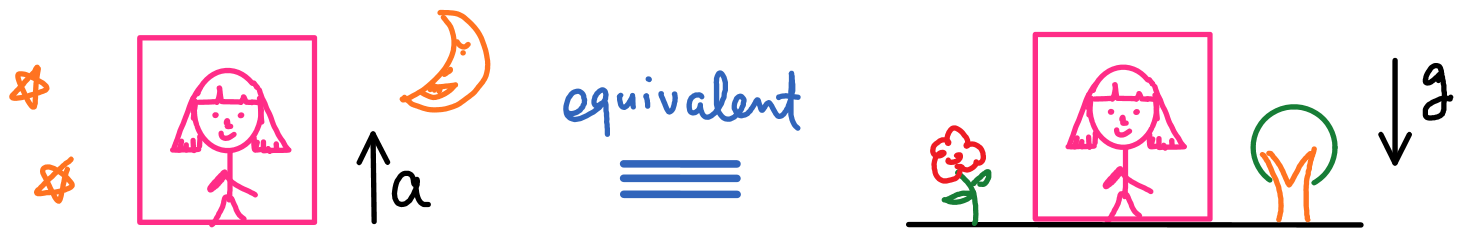
\includegraphics[width=1\textwidth]{ep}

    \tenum{
        \item The lift with constant acceleration $a$ in an environment without gravity
        \item The lift is not moving, but placed in a gravitational field $g=-a$.
    }
    \tcblower
    We added ``uniform'' to Einstein's words to make it more precise. If a gravitational field is not uniform, we can always study a small enough element of space, where the gravitational field is uniform. (How to ``patch'' these small elements together is non-trivial and will result in curved spacetime.)
    \mtextbox{Why this assumption}{Everybody can make assumptions. Why this one is special? The assumption is two-fold:
    \mtitem{
        \item Special relativity restricts our attention to inertial frames. The accelerated frame broadens the scope of relativity.
        \item Gravity gets downgraded from a ``regular'' force to something fundamentally equivalent to a fictitious inertial force.
    }}
}
This assumption indeed answered the questions: $m_I=m_G$ because inertia (acceleration) equals gravity. And gravity is special because this is the force in this fundamental assumption. 

Here we name a few simple consequences of the assumptions, and leave more surprising ones to later sections as they need more explanations.

\textbox{Uniform gravity can be cancelled by constant acceleration}{
    This is because uniform gravity $g$ is equivalent to constant acceleration $a=-g$, and constant acceleration $-g$ can be cancelled by constant acceleration $g$. 
    
    For example, one feels no gravity in free falling lifts, or satellites orbiting around the earth. These observers can in fact consider themselves as inertial frames. For these observers, the uniform gravity field can be considered non-existent (as it cannot be probed by any experiment).

    Thus (uniform) gravity is indeed special (compared to all other forces such as E\&M) -- it is as fictitious as inertial force. Its existence (or not) is observer dependent.
}
\mtextbox{Stars, light bending and lensing}{
    For a similar reason, light also bends when travelling near an object, such as a star, or a galaxy. One cannot compute the bending angle only from the equivalence principle since the gravitational field from a star is not uniform. From a calculation in general relativity, the bending angle is twice of naively applying the equivalence principle. This bending angle is the first verified prediction of general relativity (1915).
    \mnewline
    To see the light bending effect in another way: objects focus light like what a lense can do. This effect is known as \textit{gravitational lensing}\index{gravitational lensing}. Gravitational lensing is well observed and has become a powerful tool in understanding the matter distribution of our universe.
}
\textbox{Light bends in uniform gravity\index{bending of light}}{
    How light move in a uniform gravitational field? This problem may be considered as not well-defined in Newtonian mechanics as the mass of light is zero (in relativity, only zero-mass objects can move at speed of light with finite energy). But with equivalence principle, we immediately know that light bends the same way as in an accelerated environment. This explains item \ref{item:person-short} at the beginning of this part.
}

\section{Time with Uniform Gravity}

Recall that in the twin paradox, acceleration makes the physical time difference between Alice and Bob (as Alice has to accelerate to return to meet Bob again). Now acceleration equals uniform gravity, we expect that gravity should cause some time differences as well between observers. We will see that it is indeed the case.

\textbox{Higher is faster}{
    Now Alice stands higher by a vertical distance $h$ than Bob. The gravitational acceleration is $g$. Does Alice's time lapse differently from that of Bob? 
    
    To quantify ``time lapse'', consider that Alice sends two light pulses with interval $\Delta t_A$. What will be the time interval of the two pulses when Bob receives them?

    For computational simplicity, let's assume $c\Delta t_A \ll h$ and $gh\ll c^2$. The situation is illustrated in the left panel of the below figure.

    \cg{0.6}{ep_time}

    \tcblower

    To solve this problem, we make use of the equivalence principle. The system is equivalent to the situation in the right panel of the below figure: There is no gravity. But rather Alice and Bob are accelerating upwards with acceleration $a=g$. 
    
    We let $t=0$ be the time that Alice sends the first signal, and also the time that Alice and Bob has velocity $v=0$. Let the spatial separation of the light signals be $s$. Note that $s$ should be a constant because there is no gravity or other forces affecting the propagation of light.

    Wrt Alice, when she sends the signal, her velocity is $v=0$ and thus $s= c\Delta t_A$.

    \marginnote{We employed a 3rd observer C static at Bob's location to study Bob's motion wrt light. To talk about what is Bob's time interval, in fact there is time dilation effect between Bob and C. However the time dilation effect is of order $v^2/c^2$ and thus small in this analysis.}
    Wrt an observer static at Bob's location, when Bob receives the signal, his velocity is $v = a h/c$. Note that the light signals and Bob are moving towards each other. Thus $s = (c+v)\Delta t_B$. Thus
    \begin{align}
        \Delta t_A = \left ( 1 + \frac{ah}{c^2}  \right ) \Delta t_B~.
    \end{align}
    Thus, Bob finds Alice faster. The higher, the faster. If at $t=0$ Alice and Bob has the same age, later Alice will find Bob younger and Bob will find Alice older.

    This explains item \ref{item:high-fast} at the beginning of this part.
}

\mtextbox{The twin paradox again}{Now we are allowed to use the traveling twin's frame to interpret the twin paradox. The traveling twin need to accelerate before returning. If we model the acceleration to be uniform acceleration, then that corresponds to a gravitational potential due to the equivalence principle. And the static twin suddenly becomes old in this gravitational potential.}
\textbox{Time dilation with a gravitational potential}{\index{gravitational time dilation}
    More generally, for Alice and Bob in a gravitational potential $\phi$, the time dilation can be expressed in terms of their gravitational potential difference as
    \begin{align}\label{eq:gr-phi}
        dt_A = \left ( 1 + \frac{\phi_A - \phi_B}{c^2}  \right ) dt_B ~.
    \end{align}
}


\textbox{The metric for a spherical star}{\index{gravitational time dilation}
    Consider a spherical star with mass $M$. Let Bob be at $r\rightarrow \infty$, i.e. far away from the star. Then Bob does not experience gravity from the star, and has $\phi_B=0$. We can thus regard Bob's time as standard time without the star gravity: $t_B = t$.
    
    While Alice has gravitational potential $\phi_A=-GM/r$. Using Eq.~\eqref{eq:gr-phi}, we get\marginnote{Note that the gravitational field by the star is not uniform. But fortunately Eq.~\eqref{eq:gr-phi} can still be used here. And this even holds when gravity is very strong. The explanation (solving Einstein equations for the star) is beyond the scope of this short introduction.}
    \begin{align}
        dt_A = \left ( 1 + \frac{\phi_A}{c^2}  \right ) dt~.
    \end{align}
    For Alice static at a fixed position wrt the star, $d\mathbf{x}=0$, and
    \begin{align}
        \label{eq:ds2-schwarzschild}
        ds^2 = - c^2 (\mbox{proper time})^2  = - c^2 dt_A^2 
        = - \left ( 1 + \frac{2\phi_A}{c^2}  \right ) c^2 dt^2~. 
      \end{align}
      \mtextbox{Acceleration and spatial curvature}{
          Einstein noted that to reconcile accelerated frame and special relativity, the concept of curved 3d space has to be introduced. For example, consider Alice experiencing uniform circular motion, and Bob standing still at the center of the circle. Alice and Bob agrees on the radius of the circle, but not the circumference. Thus, Alice's space should be curved.
          \tcblower
          In curved space, say, a sphere, you can draw a draw a triangle and measure the sum of the inner angles. What do you get? That explains item \ref{item:inner-angle} at the beginning of this part.
      }
      In general, the coefficient in front of $d \mathbf{x}^2$ (i.e. the spatial part of the metric) is also modified. We will only give the result here: \index{Schwarzschild metric}
      \begin{align}
        \label{eq:schwarzschild}
        ds^2 = - \left ( 1 - \frac{r_s}{r}  \right ) c^2 dt^2
        + \left ( 1 - \frac{r_s}{r}  \right )^{-1} dr^2
        + r^2 \left ( d\theta^2 + \sin^2\theta d\phi^2 \right )~,
      \end{align}
      This is known as the Schwarzschild metric, describing the spacetime geometry outside a spherical symmetric star. The radius
      \begin{align}
        \label{eq:rs}
        r_s \equiv \frac{2GM}{c^2} 
      \end{align}
      is called the Schwarzschild radius. 
}

\textbox{Example: The sun}{
    To put in numbers for Eq.~\eqref{eq:rs}, if $M$ is the solar mass, then $r_s = 3$km. What does this 3km distance mean to the sun?

    \tcblower

    It does not mean anything. Because the solar radius is $r_\odot = 7\times 10^5$km. The Schwarzschild metric \eqref{eq:schwarzschild} only applies outside the star, since inside the star, the form of gravitational potential takes a different form.

    However, what if an object is so dense, that its radius is smaller than $r_s$? For example, what if an object has the same mass of the sun, but with a radius smaller than 3km?
}

\section{Black Holes}

Now imagine an object being so dense that its size is smaller than its Schwarzschild radius $r_s = 2GM/c^2$. What happens?

In fact, this is not a question living in imagination. Such dense objects -- black holes -- are real. They are detected from many observational methods, from the analysis of celestial motion to imaging its shape, to the observation of gravitational waves.

\textbox{What happens near $r=r_s$?}{
    When $r\simeq r_s$, in Eq.~\eqref{eq:schwarzschild} the time part vanishes and the spatial part blows up. What's happening there?

    Imagine 
    \mtextbox{Duality and holography}{Similar to the twin paradox, now Alice and Bob has a disagreement. Alice sees herself falling across $r_s$ but Bob sees Alice frozen at $r_s$. We will explain that they do not have a chance to meet (up to quantum subtleties which remain open questions in research) and thus nothing goes wrong.
    \mnewline
    Bob sees and describes Alice on the 2-dimensional surface $r=r_s$, while Alice sees and describes herself in a 3-dimensional volume $r<r_s$. The two descriptions \textit{may} be equivalent to each other. This conjecture is known as holography in theoretical physics as the dual descriptions are between a surface and a volume.
    }
    that Alice is staying at a distance $r$ very slightly greater than $r_s$. Gravity pulls her to fall but imagine that she is in a powerful rocket to keep her staying at a fixed $r$. And Bob locates at $r\rightarrow \infty$. For any finite interval $\Delta t_A$ according to Alice, wrt Bob:
    \begin{align}
        \Delta t_B = \Delta t_A \times \left ( 1 - \frac{r_s}{r}  \right )^{- \frac{1}{2} } \rightarrow \infty~.
    \end{align}
    Thus, Bob finds Alice frozen on the $r=r_s$ surface. In general, at $r \rightarrow r_s$, the gravitational dilation effect is so significant that time looks frozen wrt an outside observer. In this respect, if you travel close to $r\rightarrow r_s$ and then back, it's a time machine that brings you to the future.
    \tcblower
    The above is what Bob finds. But wrt Alice, she does not find $r=r_s$ very special. As at any moment, assuming that she is much smaller than $r_s$, equivalence principle tells that her acceleration cancels her gravity and she just crosses $r=r_s$ from outside to inside with finite time.
}

\textbox{An ``event horizon'' and a ``black hole''}{
    What will Bob see for the events with $r<r_s$? For example, after Alice crosses $r_s$ to reach $r<r_s$, what can Bob see about Alice?

    Nothing. 
    \mtextbox{Are black holes really black?}{
        No.
        \tcblower
        \mtitem{
            \item Theoretically, Hawking radiations from quantum gravity can come out of black holes. They are usually too dim to see.
            \item Practically, some black holes are the brightest objects in our universe -- seriously. Matter falling into the black hole (infinitely deep gravitational potential) interact with each other and emit bright radiations -- up to $40\%$ of matter energy can be converted to light. Due to the emission of infalling matter, images of black holes have been taken by arrays of radio telescopes in 2019.
        }
    }
    Due to the extreme time dilation, the light emitted at $r_s$ need infinite time to reach Bob. Bob does not have more than infinite time to wait and thus cannot see anything happening at $r<r_s$.

    As a result, $r=r_s$ is a surface to limit the events that Bob can see. Thus, $r=r_s$ is known as an \textit{event horizon}\index{event horizon}. The dense object hides inside this event horizon and thus is invisible. No light from this object can reach to outside. Thus, the object is known as a \textit{black hole}\index{black hole}. This explains item \ref{item:black-horizon} at the beginning of this part.
}
 
\textbox{``Inside'' the horizon: the future is doomed at a singularity}{
    What happens after Alice falls inside a black hole (cross the $r=r_s$ horizon)?

    Wrt Bob, he cannot expect to see Alice coming out again. Since when she crosses the horizon, it already corresponds to $t_B\rightarrow \infty$. Bob can see nothing happening later than infinity.

    But wrt Alice herself, why cannot she decide to power her rocket to escape the horizon?
    \tcblower
    To answer this question, let us take a look at the Schwarzschild metric \eqref{eq:schwarzschild}. At $r<r_s$, the metric can be rewritten as
    \begin{align}
        \label{eq:schwarzschildIn}
        ds^2 = 
        - \left ( \frac{r_s}{r} -1 \right )^{-1} dr^2
        + \left (  \frac{r_s}{r} -1  \right ) c^2 dt^2
        + r^2 \left ( d\theta^2 + \sin^2\theta d\phi^2 \right )~.
    \end{align}
    \marginnote{This explains item \ref{item:singularity} at the beginning of this part.}
    What happened? Now $dr$ is time-like and $dt$ is space-like! The time direction and one space direction have flipped their roles. For Alice, the $-r$ direction is now the time direction.

    The time direction is special since it is one-way. You can choose to move left or right in space, but have no choice but moving forward in time. Now Alice has no choice other than to move along her time direction (the direction to reduce $r$) towards $r=0$, regardless the spatial direction (now $t, \theta, \phi$) that Alice would like to travel.

    Not only Alice, but everything inside the black hole, including the dense object itself, falls towards the future at $r=0$. Their time ends here and thus it is known as a \textit{singularity}\index{singularity}. In fact, following calculations of general relativity, before reaching the singularity, every object is teared apart due to diverging tidal force near the singularity. 

    Inside a black hole, the singularity is inevitable in classical general relativity. It remains an open question how this singularity can be resolved or understood in a complete theory which can describe gravity and quantum mechanics in a consistent way (quantum gravity).
}

\section{Gravitational Waves}\index{gravitational waves}

Gravitational waves are consequences of the full theory of general relativity. Deriving them rigorously is beyond the scope here. We nevertheless build some intuitive understandings.

\textbox{Special relativity and Newtonian gravity are inconsistent}{
    What's wrong with the good old Newtonian gravity $F = G_N Mm / r^2$?

    Suppose Alice is a light year away from Bob and she waves her hand. As the position $r$ of her hands change, Bob can in principle measure a slightly different gravitational attraction from Alice \emph{immediately} -- because force needs no time to propagate in Newtonian gravity. Alice can thus encode information in how her hands move, and the information is sent to Bob immediately, which is faster than light.

    From special relativity, no information can travel faster than light. Thus, Newtonian gravity is not consistent with special relativity.

    Conceptually, replacing gravity by spacetime curvature does not solve this problem -- can the spacetime curvature change with a speed faster than light when you move your hands?
}

\mtextbox{Early history of gravitational waves}{
    Back to 1893, Oliver Heaviside noted the similarity of gravity and E\&M, and suggested that gravity may propagate in waves. But only after the estabilishment of general relativity, the discussion of gravitational waves was put into the approprate scientific framework. Einstein was the first to predict gravitational waves in 1916 based on his general relativity.
}
\textbox{What gravity can learn from E\&M?}{
    In Newtonian gravity, you can send superluminal information by waving your hands and detect the force change using $F=G_N Mm /r^2$. However, why don't E\&M have the same problem with Coulomb force $F\propto Qq/r^2$?
    \tcblower
    If we only have the Coulomb force formula and nothing else, we would have the same superluminal problem for E\&M. However, the magnetic field comes to rescue here. Once the source electric charge accelerates (you cannot encode information by inertial motion without acceleration), the time variation of the electric field produces magnetic field, and the time variation of the magnetic field produces electric field. This process happens over and over again and E\&M wave is emitted at exactly the speed of light. Also, in this way, the E\&M field can propagate by itself without the need of matter (after produced by a source) as new ``degrees of freedom''.

    The lesson: we hope that new ``degrees of freedom'' can come to rescue in gravity, similar to what magnetic field does for E\&M. Where to find those degrees of freedom?
    % Internal note: The details: gravitoelectromagnetism. See for example:
    % https://arxiv.org/pdf/gr-qc/0003115.pdf
    % https://arxiv.org/pdf/gr-qc/9912027.pdf
}

\needspace{.22\textheight}
\mtextbox{Are gravitational waves physical?}{
     The concern is that space deforms, so does rulers. So can we actually measure gravitational waves? The debate lasted for 40 years. In 1957, Feynamn (under a pseudonym of ``Mr. Smith'') argued that when gravitational waves pass, a waterdrop on a rod will move wrt the rod and thus generate heat by friction. Thus gravitational waves are physical. The observational efforts start shortly afterwards. In 2016, after decades' trail and failure, gravitatioanl waves are finally detected by the Laser Interferometer Gravitational-Wave Observatory (LIGO) using an interferometer similar to the michelson morley experiment.
}
\textbox{Optional: The dynamical metric and the gravitational waves}{
    We have shown that a static gravitational field can be described by a non-trivial metric, for example \eqref{eq:schwarzschild}. There are other components in the metric as well. The metric can be viewed as a $4\times 4$ symmetric matrix with 10 components (free functions to choose). 8 of them are already used:
    \titem{
        \item 4 to describe the response to energy and momentum of matter. The energy part is the Newtonian gravity and the momentum part is its relativistic generalization. Technically they are called the Hamiltonian (energy) and momentum constraints.
        \item 4 represents the freedom to choose coordinates. When choosing any new coordinate system $\tilde x^\mu (x)$, we expect that the physical interval should not change and thus the metric should transform accordingly.
    }
    What are the remaining 2 degrees of freedom? Happily they correspond to propagating waves of gravity, to solve the problem of Newtonian gravity. And the gravitational waves propagate at the speed of light.
}

\marginnote{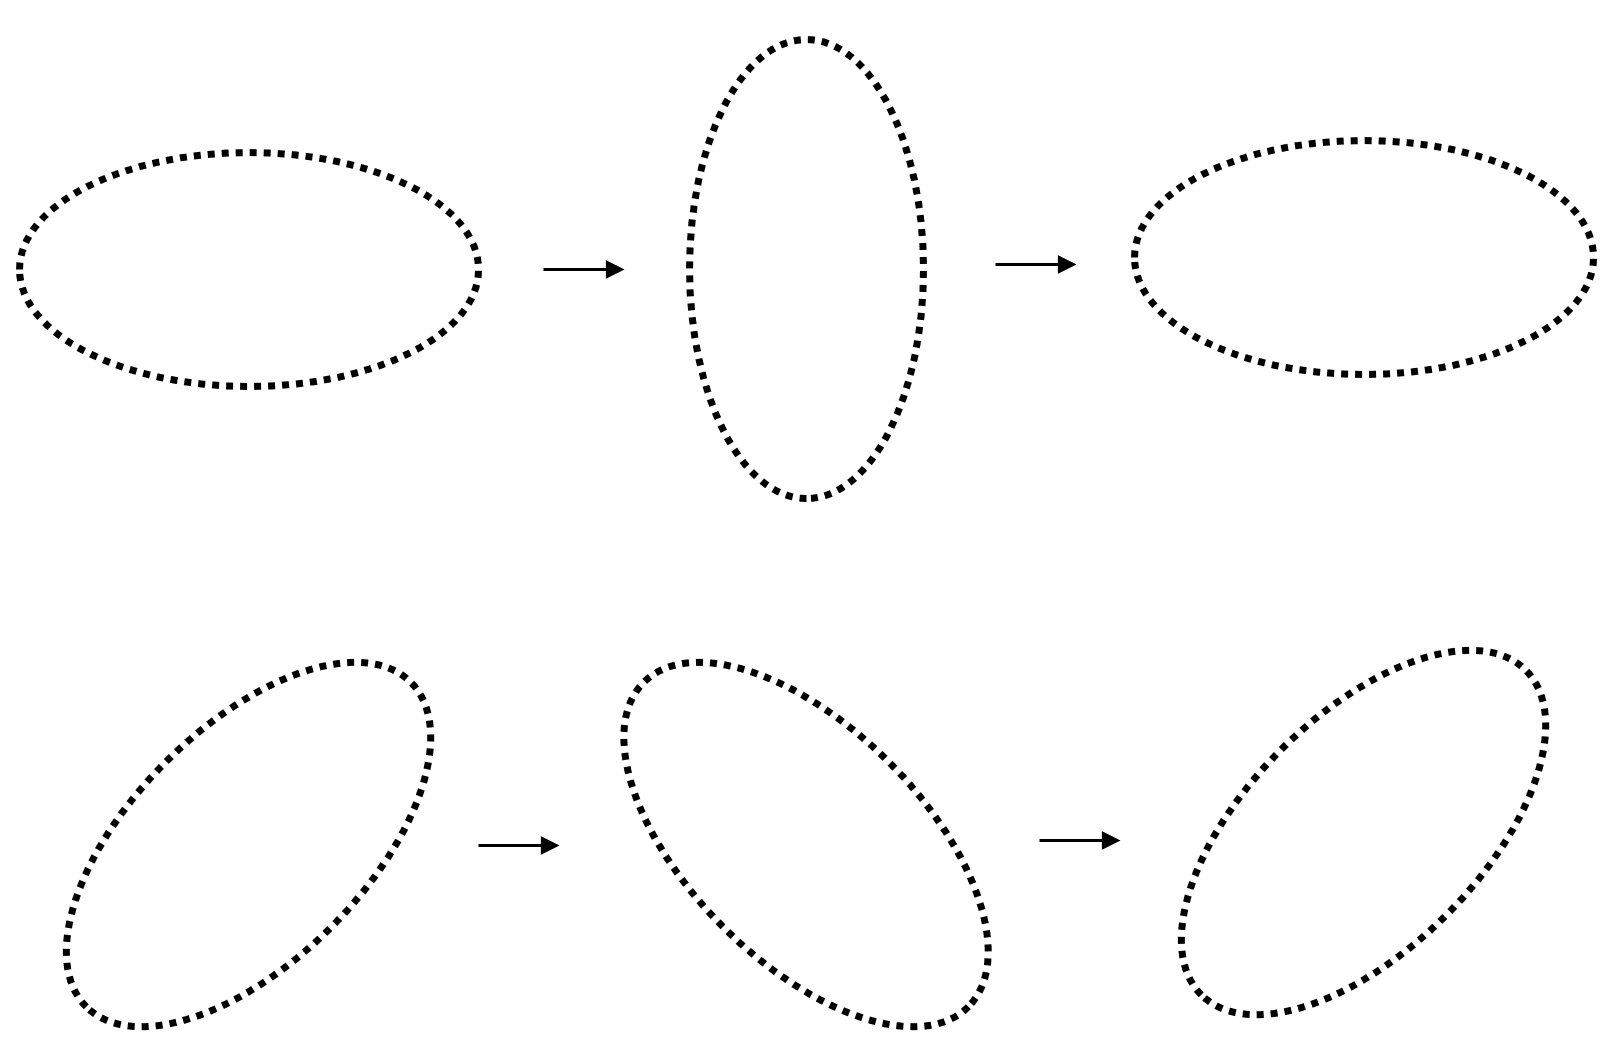
\includegraphics[width=0.35\textwidth]{gwpol}}
\textbox{What do gravitational waves look like?}{
    As we have argued, the gravitational waves are the fluctuations of spacetime, characterized by the metric. Thus, their impacts should be the distortion of distances. They travel at the speed of light and they are transverse waves (polarized perpendicular to the propagation direction). The two independent polarization modes deforms spacetime in the pattern sketched in the figure to the right.
}

\section{Epilogue: Summary and What's Next}

\textbox{A rare example in science}{
    General relativity is a very rare example in the history of modern science, that a completely new scientific framework is setup (almost) purely by logical reasoning and philosophical belief. 

    Starts from the equivalence principle, we have shown you how time becomes relative in a uniform gravitational field. Then we argued that there is a similar effect for spherical stars. And if the star is dense enough, black holes form. The black hole has an event horizon where matter (classically, without the quantum mechanical considerations) can enter but not return. From the similarity between gravity and E\&M, we have argued that gravitational waves exist as deformations of spacetime. All these can be put into precise and elegant forms with the mathematical framework of differential geometry.
}

The equivalence principle is the first observation in general relativity, but not yet the punch line. Though beyond the scope of the course, let's mention the two key concepts in general relativity:

\textbox{How space curves?}{
    How a geometry such as \eqref{eq:schwarzschild} is determined? In Newtonian gravity, we know that gravity is determined by matter distribution. Now that gravity is interpreted as geometry, geometry should be determined by matter distribution as well, at least in the Newtonian limit. The rule to determine geometry from matter distribution is the Einstein's equation. It looks like $G_{\mu\nu} = 8\pi G T_{\mu\nu}$ \index{Einstein's equations} and is the master equation of general relativity. I cannot explain it to you within the scope of this course, except mentioning that the LHS is determined by the metric $g_{\mu\nu}$ and its derivatives; and the RHS is determined by matter distribution. This is dubbed ``matter tells space how to curve.''
}

\textbox{How matter moves?}{
    How matter moves in curved space? Matter follows the geometry of spacetime. This is dubbed ``space tells matter how to move.'' Given a spacetime geometry, the motion of free-falling matter is determined by a generalized version of the twin paradox. Recall that in the twin paradox, the free observer without external force exerted has the longest proper time. We assert that, free-fall observers in general relativity still have extrema (usually longest but there are exceptions that the proper time is only longest for a selection of variations) proper times. Such extremal paths are known as geodesics. A geodesic can be interpreted in a semi-Newtonian manner as follows: the equation of a geodesic is \index{geodesic equation} $a^\mu = - \sum_{\alpha,\beta=0}^3 \Gamma^\mu_{\alpha\beta} u^\alpha u^\beta$. Here $a_\mu$ is the 4-acceleration and $u^\alpha$ is the 4-velocity. $\Gamma^\mu_{\alpha\beta}$ is a generalization of the concept of gravitational force, made from the metric and its derivatives. You may have recognized that this looks like the Newton's second law. It is at your well whether to interpret the RHS as a gravitational force, or a term in geometry to tell matter how to move. They are equivalent as implied by the equivalence principle.
}

\textbox{Is general relativity general?}{
    The above two principles are the key to general relativity, which applies to all known scales where gravity can be studied, including millimeter scales for very precise gravity experiments in the lab, to the size of the whole universe.

    Having that said, so far, we still do not understand how general relativity can be built within the framework of quantum mechanics. The efforts in searching for such a unified theory is known as ``quantum gravity''\index{quantum gravity}. Experiments have not been precise enough to probe quantum effects of gravity. But theoretical consistence between general relativity and quantum mechanics is also a well motived question, and is surprisingly hard. The current leading candidate of quantum gravity is string theory\index{string theory}, which begins with the hypothesis that elementary particles are actually strings with one spatial dimension instead of zero (zero corresponds to point particle).     
} 

\textbox{Further readings}{
    There are many great books of general relativity. Some simpler ones for beginners include \href{https://www.amazon.com/dp/0805386629/?tag=stackoverfl08-20}{Gravity: An Introduction to Einstein’s General Relativity} by Hartle and \href{https://www.amazon.com/First-Course-General-Relativity/dp/0521887054}{A First Course in General Relativity} by Schutz.
}


\section{Exercises}

1. Calculate how much faster your upstairs grow older than you. Take into account both special relativity and general relativity effects.

2. Given the precision of modern satellite navigation systems (such as BeiDou, Galileo, GLONASS or GPS), how much special relativity and general relativity effect affects the precision of these satellite navigation systems, if these factors were not taken into account?

\printindex

\end{document} 